\documentclass[11pt,preprint, authoryear]{elsarticle}

\usepackage{lmodern}
%%%% My spacing
\usepackage{setspace}
\setstretch{1.2}
\DeclareMathSizes{12}{14}{10}{10}

% Wrap around which gives all figures included the [H] command, or places it "here". This can be tedious to code in Rmarkdown.
\usepackage{float}
\let\origfigure\figure
\let\endorigfigure\endfigure
\renewenvironment{figure}[1][2] {
    \expandafter\origfigure\expandafter[H]
} {
    \endorigfigure
}

\let\origtable\table
\let\endorigtable\endtable
\renewenvironment{table}[1][2] {
    \expandafter\origtable\expandafter[H]
} {
    \endorigtable
}


\usepackage{ifxetex,ifluatex}
\usepackage{fixltx2e} % provides \textsubscript
\ifnum 0\ifxetex 1\fi\ifluatex 1\fi=0 % if pdftex
  \usepackage[T1]{fontenc}
  \usepackage[utf8]{inputenc}
\else % if luatex or xelatex
  \ifxetex
    \usepackage{mathspec}
    \usepackage{xltxtra,xunicode}
  \else
    \usepackage{fontspec}
  \fi
  \defaultfontfeatures{Mapping=tex-text,Scale=MatchLowercase}
  \newcommand{\euro}{€}
\fi

\usepackage{amssymb, amsmath, amsthm, amsfonts}

\def\bibsection{\section*{References}} %%% Make "References" appear before bibliography


\usepackage[round]{natbib}

\usepackage{longtable}
\usepackage[margin=2.3cm,bottom=2cm,top=2.5cm, includefoot]{geometry}
\usepackage{fancyhdr}
\usepackage[bottom, hang, flushmargin]{footmisc}
\usepackage{graphicx}
\numberwithin{equation}{section}
\numberwithin{figure}{section}
\numberwithin{table}{section}
\setlength{\parindent}{0cm}
\setlength{\parskip}{1.3ex plus 0.5ex minus 0.3ex}
\usepackage{textcomp}
\renewcommand{\headrulewidth}{0.2pt}
\renewcommand{\footrulewidth}{0.3pt}

\usepackage{array}
\newcolumntype{x}[1]{>{\centering\arraybackslash\hspace{0pt}}p{#1}}

%%%%  Remove the "preprint submitted to" part. Don't worry about this either, it just looks better without it:
\makeatletter
\def\ps@pprintTitle{%
  \let\@oddhead\@empty
  \let\@evenhead\@empty
  \let\@oddfoot\@empty
  \let\@evenfoot\@oddfoot
}
\makeatother

 \def\tightlist{} % This allows for subbullets!

\usepackage{hyperref}
\hypersetup{breaklinks=true,
            bookmarks=true,
            colorlinks=true,
            citecolor=blue,
            urlcolor=blue,
            linkcolor=blue,
            pdfborder={0 0 0}}


% The following packages allow huxtable to work:
\usepackage{siunitx}
\usepackage{multirow}
\usepackage{hhline}
\usepackage{calc}
\usepackage{tabularx}
\usepackage{booktabs}
\usepackage{caption}


\newenvironment{columns}[1][]{}{}

\newenvironment{column}[1]{\begin{minipage}{#1}\ignorespaces}{%
\end{minipage}
\ifhmode\unskip\fi
\aftergroup\useignorespacesandallpars}

\def\useignorespacesandallpars#1\ignorespaces\fi{%
#1\fi\ignorespacesandallpars}

\makeatletter
\def\ignorespacesandallpars{%
  \@ifnextchar\par
    {\expandafter\ignorespacesandallpars\@gobble}%
    {}%
}
\makeatother

\newlength{\cslhangindent}
\setlength{\cslhangindent}{1.5em}
\newenvironment{CSLReferences}%
  {\setlength{\parindent}{0pt}%
  \everypar{\setlength{\hangindent}{\cslhangindent}}\ignorespaces}%
  {\par}


\urlstyle{same}  % don't use monospace font for urls
\setlength{\parindent}{0pt}
\setlength{\parskip}{6pt plus 2pt minus 1pt}
\setlength{\emergencystretch}{3em}  % prevent overfull lines
\setcounter{secnumdepth}{5}

%%% Use protect on footnotes to avoid problems with footnotes in titles
\let\rmarkdownfootnote\footnote%
\def\footnote{\protect\rmarkdownfootnote}
\IfFileExists{upquote.sty}{\usepackage{upquote}}{}

%%% Include extra packages specified by user

%%% Hard setting column skips for reports - this ensures greater consistency and control over the length settings in the document.
%% page layout
%% paragraphs
\setlength{\baselineskip}{12pt plus 0pt minus 0pt}
\setlength{\parskip}{12pt plus 0pt minus 0pt}
\setlength{\parindent}{0pt plus 0pt minus 0pt}
%% floats
\setlength{\floatsep}{12pt plus 0 pt minus 0pt}
\setlength{\textfloatsep}{20pt plus 0pt minus 0pt}
\setlength{\intextsep}{14pt plus 0pt minus 0pt}
\setlength{\dbltextfloatsep}{20pt plus 0pt minus 0pt}
\setlength{\dblfloatsep}{14pt plus 0pt minus 0pt}
%% maths
\setlength{\abovedisplayskip}{12pt plus 0pt minus 0pt}
\setlength{\belowdisplayskip}{12pt plus 0pt minus 0pt}
%% lists
\setlength{\topsep}{10pt plus 0pt minus 0pt}
\setlength{\partopsep}{3pt plus 0pt minus 0pt}
\setlength{\itemsep}{5pt plus 0pt minus 0pt}
\setlength{\labelsep}{8mm plus 0mm minus 0mm}
\setlength{\parsep}{\the\parskip}
\setlength{\listparindent}{\the\parindent}
%% verbatim
\setlength{\fboxsep}{5pt plus 0pt minus 0pt}



\begin{document}



\begin{frontmatter}  %

\title{London Weather - How bad is it really?}

% Set to FALSE if wanting to remove title (for submission)




\author[Add1]{Ruan Geldenhuys}
\ead{22550801@sun.ac.za}





\address[Add1]{Stellenbosch University, Stellenbosch, South Africa}


\begin{abstract}
\small{
In order to convinve my friend not to move to the UK, I did some data
analysis on London's weather patterns. Since she is not a big reader, I
will keep my discussion to a minimum.
}
\end{abstract}

\vspace{1cm}





\vspace{0.5cm}

\end{frontmatter}



%________________________
% Header and Footers
%%%%%%%%%%%%%%%%%%%%%%%%%%%%%%%%%
\pagestyle{fancy}
\chead{}
\rhead{}
\lfoot{}
\rfoot{\footnotesize Page \thepage}
\lhead{}
%\rfoot{\footnotesize Page \thepage } % "e.g. Page 2"
\cfoot{}

%\setlength\headheight{30pt}
%%%%%%%%%%%%%%%%%%%%%%%%%%%%%%%%%
%________________________

\headsep 35pt % So that header does not go over title




\hypertarget{temperature-and-precipation}{%
\section{Temperature and
Precipation}\label{temperature-and-precipation}}

The graph below shows a breakdown of temperature and rain in London
throughout the year.

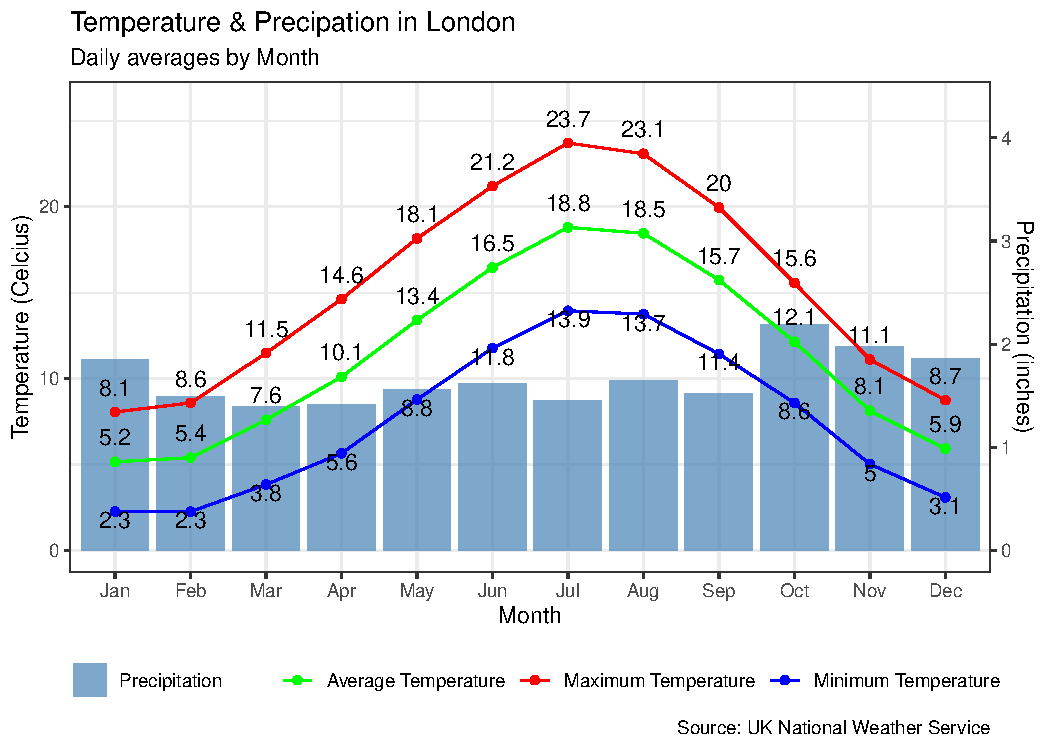
\includegraphics{Question2_files/figure-latex/unnamed-chunk-2-1.pdf}

It's clear that London is a very cold and wet place with the maximum
average temperature being 23.7 and having dearly 2 inches (50mm) of rain
all year round.

\hypertarget{sunshine-or-rather-the-lack-thereof}{%
\section{Sunshine, or rather the lack
thereof}\label{sunshine-or-rather-the-lack-thereof}}

The plot below shows the average cloud coverage in London by month.

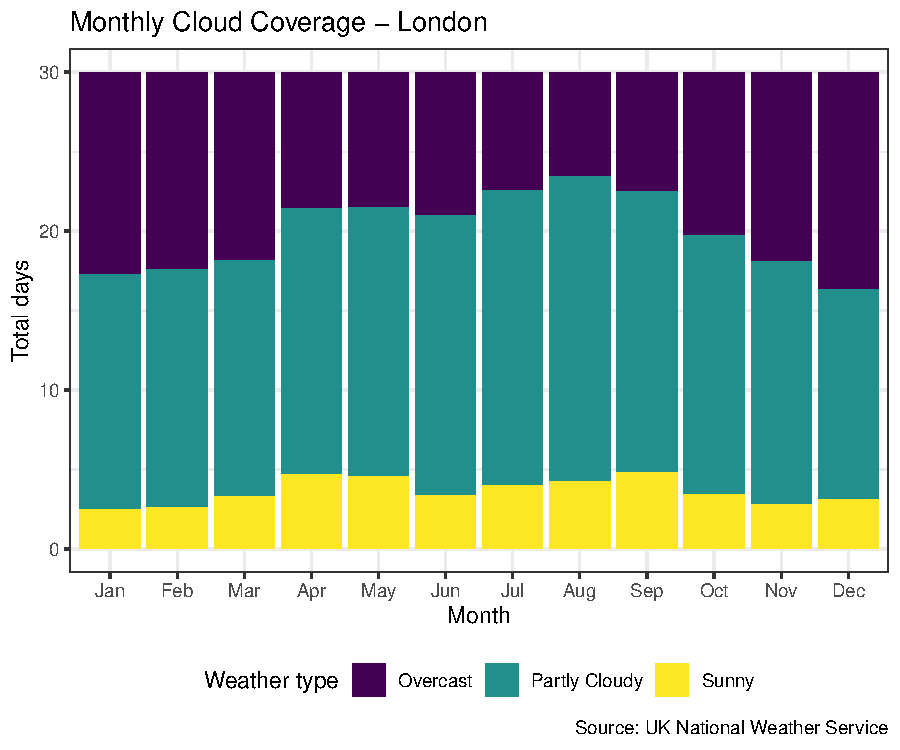
\includegraphics{Question2_files/figure-latex/unnamed-chunk-3-1.pdf}

Sunny days are few in London, as most days are partly cloudy or
overcast, as can be seen in the graph above.

\hypertarget{london-vs-cape-town}{%
\section{London vs Cape Town}\label{london-vs-cape-town}}

Using data from the Southern Africa Tourism Services Association we can
compare London and Cape Town.

\begin{table}[ht]
\centering
\caption{London vs Cape Town rain days} 
\begin{tabular}{rlrr}
  \hline
 & Month & Rainy Days (UK) & Rainy Days (CPT) \\ 
  \hline
1 & Jan & 17.80 & 3.00 \\ 
  2 & Feb & 15.60 & 2.00 \\ 
  3 & Mar & 14.60 & 3.00 \\ 
  4 & Apr & 13.40 & 4.00 \\ 
  5 & May & 12.30 & 7.00 \\ 
  6 & Jun & 12.40 & 9.00 \\ 
  7 & Jul & 11.80 & 9.00 \\ 
  8 & Aug & 12.10 & 9.00 \\ 
  9 & Sep & 12.40 & 7.00 \\ 
  10 & Oct & 15.90 & 6.00 \\ 
  11 & Nov & 17.80 & 5.00 \\ 
  12 & Dec & 17.10 & 4.00 \\ 
   \hline
\end{tabular}
\end{table}

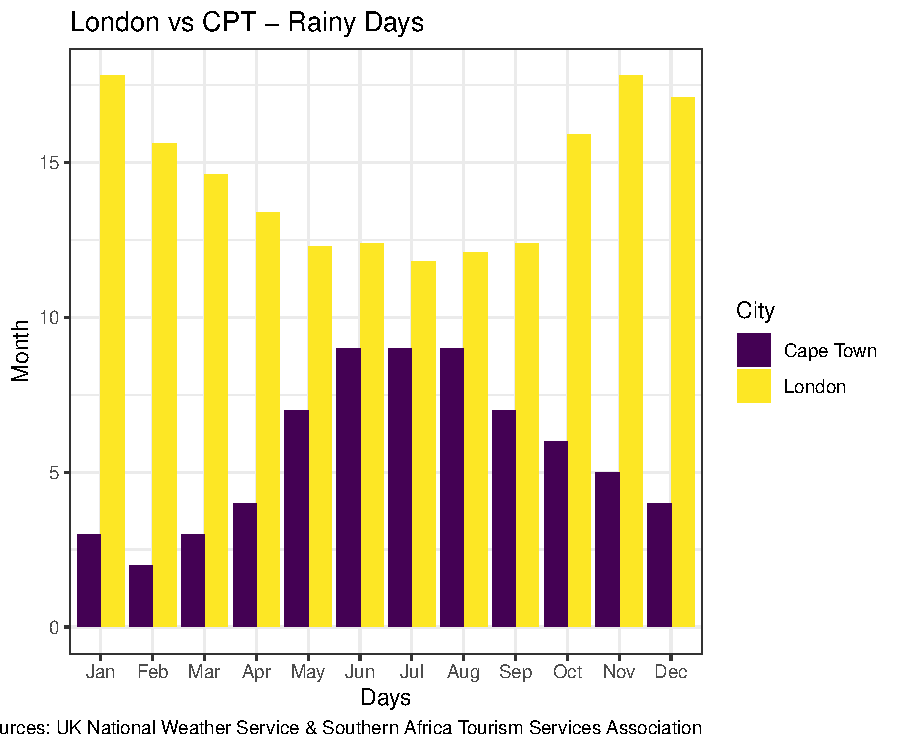
\includegraphics{Question2_files/figure-latex/unnamed-chunk-5-1.pdf}

It is clear from the table and the graph that London experiences vastly
more rain than Cape Town. London in its driest month gets more rain than
Cape Town in its wettest month.

\bibliography{Tex/ref}





\end{document}
